\chapter{Background}

\section{ASP.NET Web Forms} % (fold)
\label{sec:asp_net_web_forms}
	ASP.NET. Web Forms are the User Interface (UI) elements that give your Web applications their look and feel. Web Forms are similar to Windows Forms (ref http://msdn.microsoft.com/da-dk/library/aa983655(v=vs.71).aspx) in that they provide properties, methods, and events for the controls that are placed onto them. However, these UI elements render themselves into Html (ref http://msdn.microsoft.com/en-us/library/ms973868.aspx). When working with Web Forms you can both write markup code and write regular C\# from Code Behind when building a web application. From Code Behind there is a Page object which has different page lifecycle events which will be triggered when the page is requested. Below is an example where there is added a Button control to the Form “form1” from Code Behind (as opposed to adding the button in markup code).

	\begin{figure}
					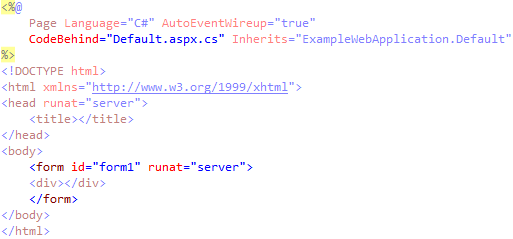
\includegraphics[width=8cm]{resources/images/Markup.png}
				\caption{Markup code in Default.aspx}
				\label{markup}
			\end{figure}

	The Default.aspx page is associated to a Code Behind file Default.aspx.cs where the pages life cycle events can be utilized. In figure \ref{codeBehind} a button control is added to the form “form1” (defined in the markup in figure \ref{markup}) in the page’s Load event.

				\begin{figure}
					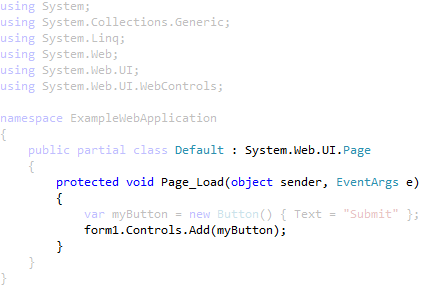
\includegraphics[width=10cm]{resources/images/CodeBehind.png}
				\caption{Default.aspx.cs Code Behind file associated to the Default.aspx page.}
				\label{codeBehind}
			\end{figure}
	The resulting web page and source will be as below (with Chrome Development Tools).

				\begin{figure}
					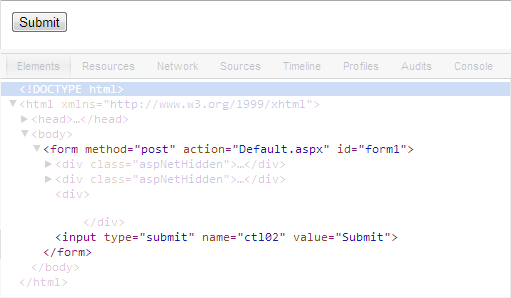
\includegraphics[width=12cm]{resources/images/Html.png}
				\caption{Resulting web page and source code of the Default.aspx page.}
				\label{html}
			\end{figure}
	There are control classes equivalent to most Html tags so in this manner one can build an entire web application from Code Behind. Some of the benefits of working from Code Behind is that you essentially achieve compile time validation of your markup code and you get to work in object oriented manner.
% section asp_net_web_forms (end)


\section{JavaScript and its Unsafe Language Features}

		\subsection{No compile time validation}
			In general enforcing correctness at compile time instead of runtime make the development process safer as some errors (e.g. syntax errors like missing semicolons) are not possible to overlook or ignore. Furthermore discovering errors as early as possible makes the debugging process easier hence compile time errors should be preferred over runtime errors. So the fact that JavaScript is an interpreted language that is not compiled makes it a less safe language.

		\subsection{Dynamic type system}
			JavaScript has a dynamic type system which in some situations make the development process faster but also less safe as some errors will not emerge at all (or maybe emerge at runtime). E.g. it is possible to by mistake add a Number value with a Boolean value without getting any warnings. In other words it is possible to forget enforcing that a variable has a specific type. This problem is increased especially when parsing external input as it is done e.g. in form validation.
		
		\subsection{Reuse of identifiers in declarations}
			JavaScript allows declaring multiple variables or functions with the same name in the same execution context without any warnings. This makes it possible by mistake to override earlier declared variables or functions. This kind of errors can be difficult and time consuming to discover because of their hidden nature.

		\subsection{No block scope}
			JavaScript’s syntax comes from C. In all other C-Like languages a block creates scope. This is not the case in JavaScript even though its block syntax suggests that it does (“The Good Parts” p. 102). This can be a source of confusion especially for programmers that are used to block scope. Scope related errors might be difficult to debug as obviously no warnings are given (since there is no block scope) when a variable from an outer block is assigned a value by mistake.

		\subsection{Many falsy values}
			JavaScript has multiple falsy values which are not interchangeable. This is another source of errors that can be difficult to discover (“The Good Parts” p. 106).

	% subsection approach_matrix (end)
